\section{La mise en place d'un cache pour les zones peuplées}
\subsection{Introduction}
Comme nous avons pu le voir dans la partie~\ref{introSolutions}, la mise en place d'un cache pour les zones peuplées permettrait d'améliorer la réactivité dans l'état (\textbf{W}). L'avantage de cette solution, même si l'issue n'était pas certaine, était de s'intéresser à une partie qui n'avait pas encore été étudiée dans Blue Banana. Nous avons donc inséré un cache pour chaque nœud de l'environnement, celui-ci va fonctionner dans la continuité de liste des voisins d'un nœud. Nous expliquerons comment nous avons inséré le cache dans le code existant, les différentes stratégies que nous avons pu mettre en place et les différents paramètres qui vont influencer le fonctionnent du cache. Nous avons aussi permis l'utilisation du cache pour aider ses voisins quand ceux-ci cherchent des nœuds.
 
\subsection{Explications de la mise en place du cache}

\subsubsection{Le fonctionnement global et la mise en place du cache dans Blue Banana}
Le fonctionnement global du cache consiste à garder en mémoire un certains nombre de nœuds qui faisait parti de la liste des voisins. Ainsi comme les mouvements de l'avatar sont désordonnés, il est possible qu'il retourne vers des nœuds qu'il vient de quitter. 
\par Sur la figure~\ref{cacheW}, nous pouvons voir les principales étapes du fonctionnement du cache. Au départ le cache et la liste des voisins sont remplis de différents nœuds. A l'étape 2, le nœud courant (rouge) se déplace et trouve des nouveaux voisins, ceux-ci sont insérés à sa liste des voisins. Deux nœuds sont alors déplacés vers le cache, ce qui pousse deux nœuds hors du cache. A la dernière étape, le nœud courant revient vers une zone qu'il connait (nous détaillerons après le mécanisme de recherche dans le cache) et il trouve deux nœuds dans son cache qui pourraient lui servir pour reconstruire son voisinage. Deux nœuds du cache sont alors insérés dans la liste des voisins du nœud courant, ce qui envoie deux nœuds de cette liste vers le cache. Dans cette exemple, plusieurs nœuds peuvent se déplacer en même temps, ce qui est le cas dans une seule des solutions de cache mise en place.
	\begin{figure}[!h]
        \centering
        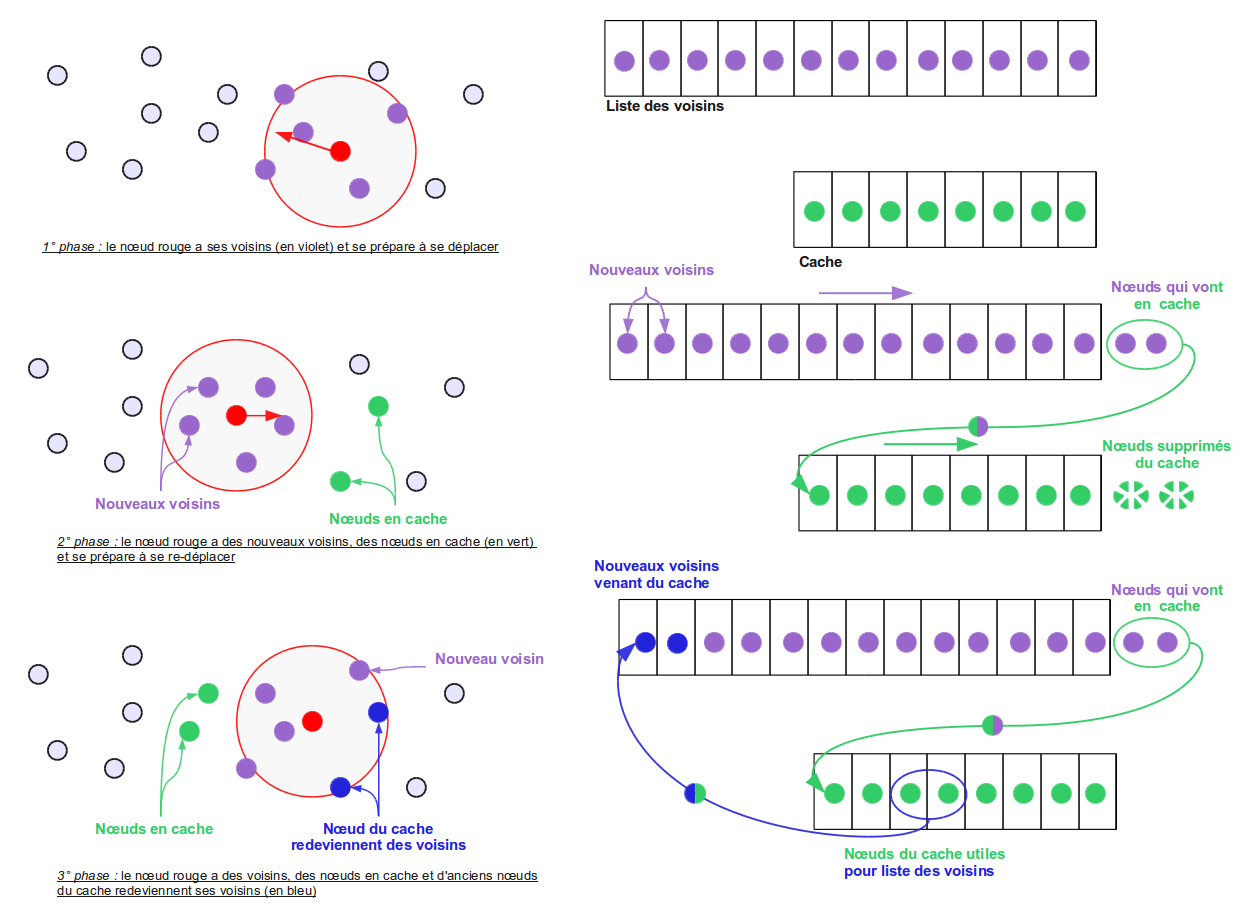
\includegraphics[scale=0.35]{./Ressources/Images/cacheWextends.png}
        \caption{Exemples du fonctionnement global du cache}
        \label{cacheW}
        \end{figure} 
\par Cette solution permet d'économiser des messages de découverte des voisins (SEARCH) dans le cas de changements de direction fréquents. Il doit aussi nous permettre d'économiser des messages de connexions et de déconnexion. Nous verrons dans la partie~\ref{resObsCache} les différents gains de la mise en place du cache, mais aussi les limites de celui-ci. Le cache est donc le prolongement de la liste des voisins pour nœud, mais contrairement à celui-ci , il n'est pas à jour, car un nœud est ajouté dans le cache avec les dernières informations que nous avions quand il était dans la liste des voisins. Nous avons donc mis en place un système de mise à jour du cache, pour avoir des informations les plus exactes possibles sur chaque nœud. Mais ce système va coûter cher en nombre de messages, et cela est encore plus vrai plus le cache est grand. Un mécanisme de datation des éléments du cache permet de savoir depuis quand date les informations de chacun. Ce mécanisme nous permet de contacter un nœud pour savoir s'il se trouve toujours à peu près au même endroit, et ainsi l'ajouter ou non à notre voisinage. Ces paramètres sont en option et nous verrons dans la partie~\ref{resObsCache} quelles sont les meilleures combinaisons d'options et si elles sont toutes utiles ou non.

\subsubsection{Les différentes versions du cache}

Deux versions, pour le fonctionnent du cache, ont été testées durant la phase de codage. Nous parlons ici de la gestion des données dans le cache et non de la recherche dans celui-ci qui se fera juste après. Au départ le cache était géré selon le principe \textit{First In First Out}, la gestion du cache ne tenait pas compte des mises à jours.  Ces mises à jour peuvent avoir lieu lors d'une requête en échec vers un nœud du cache.Le nœud ayant trop bougé est alors mis à jour dans le cache. Une gestion du cache en fonction de la localité a aussi été mise en place, ce qui permet de faire sortir du cache les nœuds les plus éloignés de la position actuelle du nœud.
\par Deux implémentations ont aussi été testées pour la recherche dans le cache, l'une renvoie un résultat et l'autre renvoie plusieurs nœud à ajouter. Les tests montrent que la deuxième implémentation donne de meilleurs résultats (voir chapitre~\ref{resObsCache}).


\subsubsection{La modification du code existant pour insérer la recherche dans le cache}

 Avant de regarder les algorithmes de recherche dans le cache, nous allons vous expliquer comment ils sont appelés et quelles sont les modifications introduites par rapport au code original. Lorsqu'un nœud rentre dans la fonction \textit{solipsisRecoverTopology} si le nœud est dans l'état \textbf{Wandering} alors on passe dans la fonction \textit{MaintainTopology}, sinon on effectue le traitement normal. Nous pouvons voir ci-dessous une partie du code de la fonction MaintainCache. Pour commencer, nous testons l'état de l'entité appelante, ensuite en fonction de la stratégie, nous faisons un traitement particulier. Nous nous concentrerons sur la stratégie de base qui ajoute un seul nœud. La fonction de recherche nous renvoie donc un résultat. S'il n'est pas nul et que sa date de mise à jour n'est pas trop ancienne, nous enlevons le nœud du cache, ajoutons le nœud à la liste des voisins et renvoyons 1 à la fonction appelante pour lui signifier que le traitement à été fait. Ensuite en fonction de la valeur de l'option \textit{contact\_node}, nous contactons ou non le nœud renvoyé par la fonction de recherche. Nous faisons ceci pour savoir s'il a beaucoup bougé depuis le dernier moment où nous l'avons vu. Nous retournons 0 pour signifier à la fonction appelante qu'aucun nœud n'a été ajouté et qu'elle peut faire le traitement de base.

\lstset{numbers=left,basicstyle=\scriptsize, numberstyle=\tiny, stepnumber=5, numbersep=5pt}

\lstinputlisting[title={Partie du code de la fonction MaintainCache},label={codeMaitainTopology}]{./Ressources/Documents/MaintainTopology.java}



\subsubsection{Les algorithmes de recherche dans le cache}
\par Nous allons expliquer comment nous recherchons les données dans le cache, et nous détaillerons les différentes pistes que nous avons testé dans un ordre chronologique. Tout d'abord nous avons sélectionner les nœuds en terme de distance. L'idée  était de récupérer les plus proches de notre nouvelle position. Cette solution était assez simple à mettre en place, mais nous pensions que les résultats seraient meilleurs si nous prenions en compte la capacité d'un nœud à aider à refaire l'enveloppe connexe du nœud courant. Nous avons alors implémenté une solution qui rendait un résultat positif si un nœud dans le cache permettait de reconstruire l'enveloppe du nœud (voir schéma~\ref{schemaEnvelopCache}). Cette solution a même été agrémentée d'un test si le nœud faisait avancer positivement l'enveloppe connexe mais ne la reconstruisait pas immédiatement.

	\begin{figure}[!h]
        \centering
        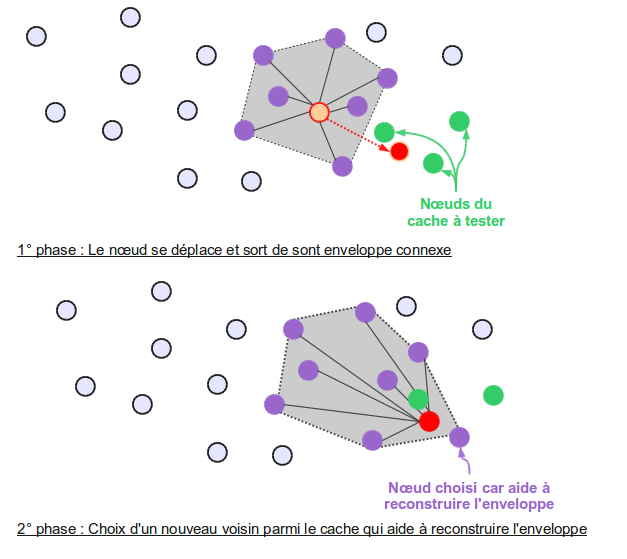
\includegraphics[scale=0.45]{./Ressources/Images/cacheReconstructEnvelop.png}
        \caption{Schéma montrant la solution de recherche dans le cache aidant à reconstruire l'enveloppe}
        \label{schemaEnvelopCache}
        \end{figure}
\par Le problème de cette solution est qu'elle privilégiait l'enveloppe connexe à la propriété de \textit{Local Awareness}. Car nous pouvons nous retrouver dans la situation, comme dans la figure~\ref{schemaEnvelopCache}, où un nœud ne fait pas parti de la liste des voisins alors qu'il se trouve dans l'enveloppe connexe. Cette solution nous donnait donc des résultats, pour les propriétés de Solipsis, qui étaient moins bons que la version sans le cache.  

\par Nous sommes alors revenus à une solution ressemblant à la première solution que nous avions mise en place. Chaque nœud comporte une zone de connaissance, nous avons donc décidé de nous servir de cette dernière pour réaliser les conditions dans la fonction de recherche. La fonction de recherche regarde si un nœud du cache est dans la zone de connaissance du nœud courant. Si plusieurs correspondent un système pour choisir aléatoirement est mis en place, comme dans la recherche de voisin original. Une autre fonction qui recherche en prenant en compte la région géométrique a aussi été mise en place, les résultats sont équivalents à la version avec la zone de connaissance.


\subsubsection{La mise en place de l'aide aux voisins grâce au cache}

Le cache d'un nœud va donc lui servir pour essayer de connaitre son environnement plus rapidement, mais il pourrait aussi aider les voisins du nœud. Dans cette optique, l'aide aux voisins a été mise en place. Ceci permet au cache d'avoir une autre utilisation, ce qui pourrait permettre d'économiser quelques autres messages. 
\par Lorsqu'un nœud cherche des voisins, il envoie un message SEARCH (voir schéma~\ref{schemaHelpCache}). Il suffit donc d'insérer une recherche dans le cache au bon endroit dans la fonction de traitement de ce message. Nous insérons donc, dans la fonction \textit{processSearchMsg}, une fonction de recherche dans le cache. Le nœud va tout d'abord regarder dans sa liste des voisins et si aucun ne correspond, nous regardons dans le cache si un nœud peut correspondre à la requête. La recherche dans le cache se fait, de façon similaire à une recherche dans le cache pour un nœud local, en utilisant la zone de connaissance que l'on aura préalablement transmis dans le message.

	\begin{figure}[!h]
        \centering
        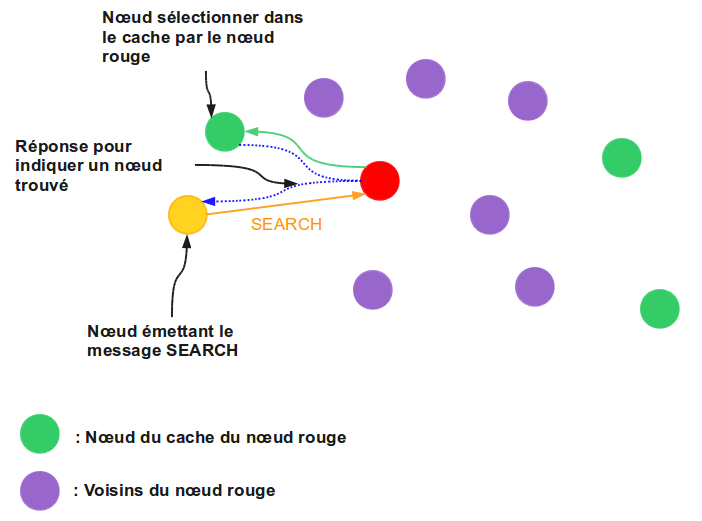
\includegraphics[scale=0.4]{./Ressources/Images/cacheHelp.png}
        \caption{Schéma montrant l'aide du cache pour le traitement d'un message SEARCH}
        \label{schemaHelpCache}
        \end{figure}

\subsection{Résultats et observations sur le cache}
\label{resObsCache}

Nous allons présenter les différents résultats sur le cache. Nous comparerons chaque version avec une version de base où l'on ne trouve ni cache ni prefetch, et avec une version avec le prefetch implémenté dans Blue Banana.
Les principales métriques pour comparer les différents résultats sont la cohérence de la topologie et le nombre de messages qui sont exprimés en fonction de la mobilité des avatars. Le calcul de la cohérence de la topologie consiste à mesurer, à chaque instant, le nombre de nœud qui sont dans la zone de connaissance d'un autre nœud mais qui ne fait pas parti des voisins de ce dernier.

\subsubsection{Résultats avec une première configuration du cache}
\par Tout d'abord, nous allons regarder le nombre de cache Hit et Miss pour le cache normal. Il s'agit de voir le taux de réussite du cache et donc si ce mécanisme est souvent utlisé. Dans ces premiers résultats, le cache est configuré de tel sorte qu'il n'utilise pas l'aide aux voisins, qu'il ne contacte pas un nœud du cache s'il est trop vieux. Cette configuration ne va récupérer que les nœuds du cache qui sont très proches et qui ont été ajoutés au cache récemment (voir tableau ci dessous). La taille du cache correspond au nombre de nœud qu'il peut contenir, la limite de distance correspond à la distance à partir de laquelle nous ne récupèrerons pas le nœud. La limite de temps est la différence maximum qu'il doit y avoir entre le temps courant et la date de rafraichissement du nœud dans le cache (généralement l'ajout de celui-ci dans le cache). 
\begin{table}[!h]
  \begin{center}
    \begin{tabular}{|c|c|}
      \hline
      Paramètre & Valeur\\
      \hline
      Taille du cache & 25\\
      Limite de distance &  1500\\
      Limite de temps & 1500\\
      Contact Nœud & Faux\\
      Mise à jour du cache & Faux\\
      Aide aux voisins & Vrai\\
      \hline
    \end{tabular}
  \end{center}
  \label{tab:config1}
  \caption{Tableau montrant les valeurs utilisées pour la configuration n°1}
\end{table}


\par Nous pouvons voir que plus la mobilité augmente plus le nombre de cache Hit augmente et le nombre de cache Miss diminue (voir figure~\ref{courbesHitMiss:config1}). Cela est dû au fait que plus la mobilité augmente plus le cache aura des entrées récentes, car les nœuds vont changer de direction plus souvent et plus rapidement. Notre politique de cache ne prenant en compte que des nœuds récemment ajoutés au cache, les résultats en terme de cache Hit sont bien meilleurs. Nous pouvons aussi noter qu'il ya de moins en moins d'accès au cache car la somme des Hit et des Miss diminue, cela est du au fait que de plus en plus de nœuds sont dans un état \textbf{T}. 

	\begin{figure}[!h]
        \centering
        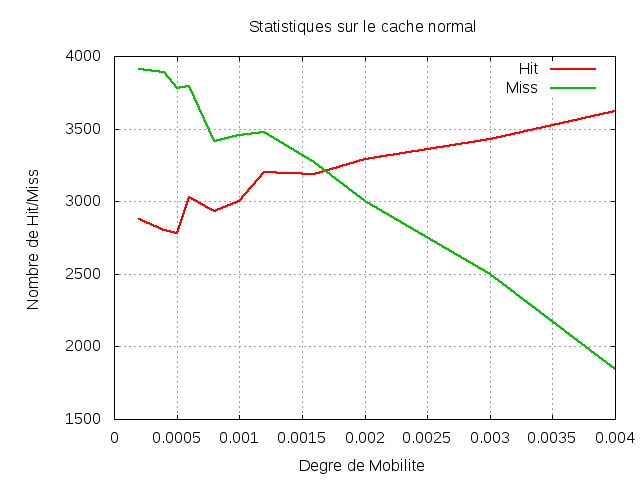
\includegraphics[scale=0.5]{../CacheCode/SolipsisPeersim/resultats/Courbes/Courbes_Final_Rapport/Cache_Stats_Normal.png}
        \caption{Schéma montrant les caches Hit et caches Miss pour le cache normal}
        \label{courbesHitMiss:config1}
        \end{figure}
\newpage
\par Ensuite nous pouvons observer le nombre de messages en fonction du degré de mobilité (voir figure~\ref{courbesNbMessCache:config1}). Les deux versions du cache vont nous permettre d'économiser des messages car lors d'un cache Hit nous ne faisons pas le traitement de base qui provoquait l'envoie d'un message. Le traitement du cache se fait sans coût en terme de message. Si l'on fait le traitement de base après le passage dans le cache, un gain en nombre de message sera tout de même réalisé. Ce gain résulte du fait que le nœud connaîtra mieux son environnement et la prochaine fois qu'il devra entrer dans la fonction \textit{MaintainCache} sera retardée. Ces observations sont les mêmes pour le cache à réponse simple et le cache à réponse multiple.  


	\begin{figure}[!h]
        \centering
        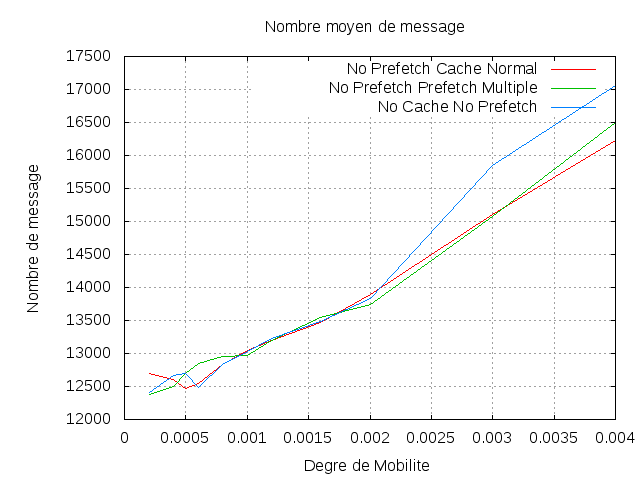
\includegraphics[scale=0.5]{../CacheCode/SolipsisPeersim/resultats/Courbes/Courbes_Final_Rapport/Nombre_Messages_Caches.png}
        \caption{Schéma montrant le nombre de messages}
        \label{courbesNbMessCache:config1}
        \end{figure}

Nous allons maintenant observer la cohérence de la topologie avec les différentes versions du cache. PROBLEME AVEC CACHE SIMPLE. La version du cache fonctionnant avec une recherche renvoyant plusieurs nœuds donne des résultats meilleurs que la version de base (sans cache et sans prefetch). A FINIR

	\begin{figure}[!h]
        \centering
        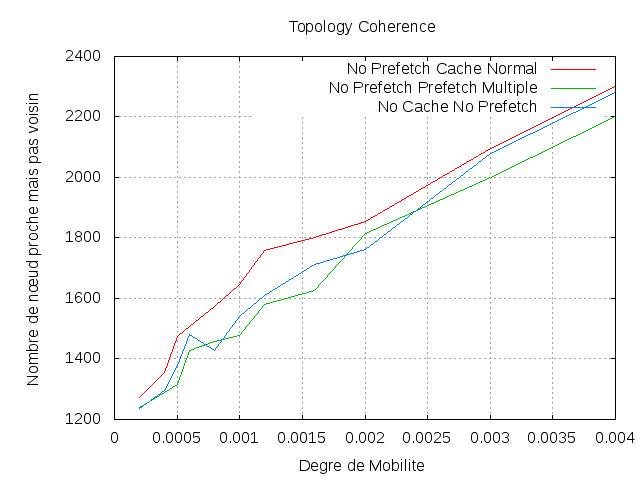
\includegraphics[scale=0.5]{../CacheCode/SolipsisPeersim/resultats/Courbes/Courbes_Final_Rapport/Topology_Coherence_Caches.png}
        \caption{Schéma montrant la cohérence de la topologie}
        \label{courbesTopoCohCache:config1}
        \end{figure}

\newpage
\subsubsection{Résultats avec une seconde configuration du cache}

\begin{table}[!h]
  \begin{center}
    \begin{tabular}{|c|c|}
      \hline
      Paramètre & Valeur\\
      \hline
      Taille du cache & 25\\
      Limite de distance &  3500\\
      Limite de temps & 3000\\
      Contact Nœud & Vrai\\
      Mise à jour du cache & Faux\\
      Aide aux voisins & Vrai\\
      \hline
    \end{tabular}
  \end{center}
  \label{tab:config2}
  \caption{Tableau montrant les valeurs utilisées pour la configuration n°3}
\end{table}



A FINIR ??


\subsubsection{Résultats avec une troisième configuration du cache}

\begin{table}[!h]
  \begin{center}
    \begin{tabular}{|c|c|}
      \hline
      Paramètre & Valeur\\
      \hline
      Taille du cache & 25\\
      Limite de distance &  3500\\
      Limite de temps & 3000\\
      Contact Nœud & Vrai\\
      Mise à jour du cache & Vrai\\
      Aide aux voisins & Vrai\\
      Fréquence de mise à jour & 5000\\
      \hline
    \end{tabular}
  \end{center}
  \label{tab:config3}
  \caption{Tableau montrant les valeurs utilisées pour la configuration n°3}
\end{table}


A FINIR ??


\subsection{Conclusion et perspectives du cache} 

La mise en place du cache permet d'économiser des messages et cela est d'autant plus vrai que la mobilité est grande. Un des problèmes dans les résultats du cache est qu'une version simple fait perdre de la cohérence de topologie, et ce même si l'on effectue aussi le traitement de base. WHY ? RE TESTER et MODIFIER CODE?

